\chapter{Strings}

\section{Hashing}

    Hashing consists in generating a Polynomial for the string, 
    therefore, assigning each distint string to a specific numeric value
    In practice, there will always be some collisions:

    Probability of colision: = $ \frac{n^2}{2 m} $

    n = Comparissons, m = mod size

    when using multiple mods, they multiply: m = m1 * m2

    \kactlimport{hashing.cpp}

\section{Z-Function}

    Suppose we are given a string \textit{s} of length \textit{n}. 
    The Z-function for this string is an array of length \textit{n} where the \textit{i-th}
    element is equal to the greatest number of characters starting from the position \textit{i}
    that coincide with the first characters of \textit{s} (the prefix of \textit{s})

    The first element of the Z-function, z[0], is generally not well defined. 
    This implementation assumes it as z[0] = 0. 
    But it can also be interpreted as z[0] = n (all characters coincide).

    Can be used to solve the following simples problems:

    \begin{itemize}
		\item Find all ocurrences of a pattern p in another string s. 
        (p + '\$' + s) (z[i] == p.size())

        \item Find all borders. A border of a string is a prefix that is also a suffix of 
        the string but not the whole string. 
        For example, the borders of abcababcab are ab and abcab. (z[8] = 2, z[5] = 5)
        (z[i] = n-i)

        \item Find all period lengths of a string. 
        A period of a string is a prefix that can be used to generate the whole string by repeating
        the prefix. The last repetition may be partial. For example, the periods of \textit{abcabca} 
        are \textbf{abc}, \textbf{abcabc} and \textbf{abcabca}.

        It works because (z[i] + i >= n) is the condition when the common characters of z[i] in addition
        to the elements already passed, exceeds or is equal to the end of the string. For example:

        \textit{abaababaab}
        z[8] = 2

        \textbf{abaababa} is the period; the remaining (z[i] characters) are a prefix of the period; 
        and when all these characters are combined, it can form the string (which has n characters).

	\end{itemize}

    \kactlimport{zfunction.cpp}

\section{KMP}

    KMP stands for Knuth-Morris-Pratt and computes the prefix function.

    You are given a string $s$ of length $n$. 
    The prefix function for this string is defined as an array $\pi$ of length $n$, 
    where $\pi[i]$ is the length of the longest proper prefix of the substring $s[0 \dots i]$
    which is also a suffix of this substring. A proper prefix of a string is a prefix that
    is not equal to the string itself. By definition, $\pi[0] = 0$.

    For example, prefix function of string \textit{"abcabcd"} is $[0, 0, 0, 1, 2, 3, 0]$,
    and prefix function of string \textit{"aabaaab"} is $[0, 1, 0, 1, 2, 2, 3]$.

    \kactlimport{kmp.cpp}

\section{Suffix Array} 

    The suffix array is the array with size n, whose values are the indexes 
    from the longest substring (0) to the smallest substring (n) after ordering it lexicographically. 
    Example:
    
    \begin{center}
    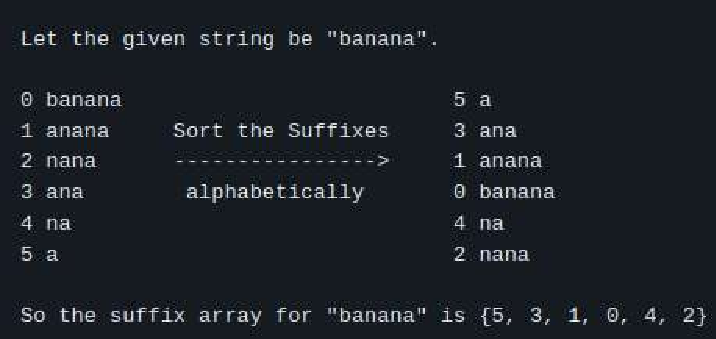
\includegraphics[width=90mm]{content/strings/suffix-array.pdf}
    \end{center}

    Note that the lenght of the string i is: {s.size()-sa[i]}

    \kactlimport{suffix-array.cpp}

    Kasai generates an array of size n (like the suffix array), 
    whose values indicates the lenght of the longest common prefix beetwen sa[i] and sa[i+1]

    \kactlimport{kasai.cpp}

    \textbf{Problems that can be solved:}

    Numbers of Distinct Substrings: (n*(n+1))/2 - lcp[i] {for all i}

    Longest Repeated Substring: biggest lcp[i]. The position can be found in sa[i]

    Find how many distinct substrings there are for each len in [1:n]: Use delta encoding and the fact that lcp[i] counts the repeated substring between s.substr(sa[i]) and s.substr(sa[i+1]), which are the substrings corresponding to the commom prefix.

    Find the k-th distinct substring: 

    % string s; cin >> s;
    % ll n = s.size();
    
    % auto sa = suffix_array(s);
    % auto lcp = kasai(s, sa);

    % ll k; cin >> k;

    % for(ll i=0; i<n; i++) {
    %     ll len = n-sa[i];
    %     if (k <= len) {
    %         cout << s.substr(sa[i], k) << endl;
    %         break;
    %     }
    %     k += lcp[i] - len;
    % }

\section{Manacher}

    Manacher's Algorithm is used to find all palindromes in a string.

    For each substring, centered at i, find the longest palindrome that can be formed.
    
    Works best for odd size string, so we convert all string to odd ones
    by adding and extra characters between the original ones

    Therefore, the value stored in the vector cnt is actually palindrome-len + 1.

    \kactlimport{manacher.cpp}

\section{Booth}

    An efficient algorithm which uses a modified version of KMP to compute the
    least amount of rotation needed to reach the \textbf{lexicographically minimal string rotation}.

    A rotation of a string can be generated by moving characters one after another from beginning to end.
    For example, the rotations of \textit{acab} are \textit{acab}, \textit{caba}, \textit{abac}, and \textit{baca}.

    \kactlimport{booth.cpp}